\documentclass[a4paper,12pt]{article}

% Import the deliverable package from common directory
\usepackage{../common/deliverable}

% Tell LaTeX where to find graphics files
\graphicspath{{../common/logos/}{./figures/}{../}}

\usepackage{xspace}
\usepackage{subcaption}
\usepackage{amsmath}
\usepackage{todonotes}
\usepackage{pgfplots}
\usepackage{pgfplotstable}
\pgfplotsset{compat=1.15}

% GitHub shortcuts for dealii/dealii issues and pull requests
\newcommand{\issue}[1]{\href{https://github.com/dealii/dealii/issues/#1}{\##1}}
\newcommand{\pr}[1]{\href{https://github.com/dealii/dealii/pull/#1}{PR:\##1}}

\makeatletter
\definecolor{gnuplot@orange}{RGB}{229,158,0}
\definecolor{gnuplot@purple}{RGB}{148,0,212}
\definecolor{gnuplot@lightblue}{RGB}{87,181,232}
\definecolor{gnuplot@green}{RGB}{0,158,115}
\definecolor{gnuplot@darkblue}{RGB}{0,115,179}
\definecolor{gnuplot@yellow}{RGB}{240,227,66}
\pgfplotscreateplotcyclelist{colorGPL}{%
gnuplot@darkblue,every mark/.append style={fill=gnuplot@darkblue!80!black},mark=o\\%
red!80!white,every mark/.append style={fill=red!80!black},mark=square\\%
gnuplot@green,every mark/.append style={fill=gnuplot@green!50!black},mark=otimes*\\%
gnuplot@orange,every mark/.append style={fill=gnuplot@orange!80!black,mark size=2.5pt},mark=x\\%
gnuplot@purple,mark=diamond\\%
black,densely dashed,every mark/.append style={solid,fill=gnuplot@darkblue!80!black},mark=square*\\%
gnuplot@lightblue,densely dashed,every mark/.append style={solid,fill=gnuplot@lightblue!30!black},mark=triangle*\\%
red!80!white,densely dashed,every mark/.append style={solid,fill=red!40!white},mark=oplus*\\%
}
\makeatother

% Set the deliverable number (without the D prefix, it's added automatically)
\setdeliverableNumber{1.7}

% Begin document
\begin{document}

% Create the title page with the title as argument
\maketitlepage{Improvements to deal.II}

\newpage

% Main Table using the new environment and command
\begin{deliverableTable}
    \tableEntry{Deliverable title}{Improvements to deal.II}
    \tableEntry{Deliverable number}{D1.7}
    \tableEntry{Deliverable version}{[Version number]}
    \tableEntry{Date of delivery}{[Planned date]}
    \tableEntry{Actual date of delivery}{[Actual date]}
    \tableEntry{Nature of deliverable}{Report}
    \tableEntry{Dissemination level}{Public}
    \tableEntry{Work Package}{WP1}
    \tableEntry{Partner responsible}{UNITOV}
\end{deliverableTable}

% Abstract and Keywords Section
\begin{deliverableTable}
    \tableEntry{Abstract}{}
    \tableEntry{Keywords}{}
\end{deliverableTable}

\newpage

\begin{documentControl}
    \addVersion{0.1}{21/02/2026}{Marco Feder}{Initial draft}
    \addVersion{0.2}{22/02/2026}{Marco Feder}{Polygonal discretization module section}
    \addVersion{0.3}{23/02/2026}{Marco Feder}{Integration and preliminary results for PSCToolkit}
    \addVersion{0.4}{23/02/2026}{Chiara Puglisi}{Preliminary results
      with advanced features in MUMPS}
    \addVersion{0.5}{25/02/2026}{Luca Heltai}{Integration of VTK utilities and new tutorial}
\end{documentControl}

\subsection*{{Approval Details}}
Approved by: [Name] \\
Approval Date: [Date]

\subsection*{{Distribution List}}
\begin{itemize}
    \item [] - Project Coordinators (PCs)
    \item [] - Work Package Leaders (WPLs)
    \item [] - Steering Committee (SC)
    \item [] - European Commission (EC)
\end{itemize}

\vspace*{2cm}

\disclaimer

\newpage

\tableofcontents % Automatically generated and hyperlinked Table of Contents

\newpage

\section{{Introduction}}



\subsection{{Purpose of the Document}}


\subsection{{Structure of the Document}}
\begin{itemize}
    \item Section \ref{sec:section2}: Pre-exascale capabilities of deal.II
    \item Section \ref{sec:section3}: Pre-exascale modules of deal.II
    \item Section \ref{sec:section4}: Polygonal discretization module
    \item Section \ref{sec:section5}: Integration of PSCToolkit
    \item Section \ref{sec:section6}: Integration of MUMPS
\end{itemize}

\newpage


\section{{Extending and improving the exascale capabilities of deal.II}}
\label{sec:section1}


\subsection{{Bakeoff kernels}}
    We have expanded the Matrix-Free Operator evaluation framework by improving Kokkos-based Bake-Off kernels with different variants.
    These variants, which build upon the groundwork of Deliverables 1.3 and 3.2 benchmark implementations, leverage two-dimensional thread structures to
    maximize data locality and hardware efficiency. These implementations, available at dealii-X benchmarks repository \footnote{\url{https://github.com/dealii-X/benchmarks}} under sum\_factorization folder,
    utilize a two-dimensional thread block structure to significantly enhance thread-wise data locality and throughput. Additionally,
    C++ templates are leveraged to enable aggressive compile-time optimizations, including loop unrolling.

    Performance evaluations were conducted on the NVIDIA GH200 Grace Hopper Superchip, which integrates an ARM-based 72-core Grace CPU with a Hopper architecture GPU.
    This architecture utilizes HBM3e memory, providing a high-bandwidth memory subsystem. Using the Kokkos-based Stream Triad benchmark, we measured an 
    effective memory bandwidth of 3.65 TB/s, which serves as a reference point for the high-bandwidth capabilities of the GH200 platform.

    As illustrated in Figure \ref{fig:N_BK1_BK5}, preliminary results indicate that BK1 and BK5 achieve peak throughputs approaching 90 GDOF/s (billion degrees of freedom per second)
    at specific polynomial orders using single-precision arithmetic (FP32). In contrast, BK3 (see Figure \ref{fig:N_BK3}) plateaus at approximately 25 GDOF/s. A consistent trend across these kernels is the underperformance 
    of low-order elements ($p=1, p=2$). This bottleneck is primarily attributed to low occupancy; the low thread count per thread block fails to saturate the standard 32-thread warp,
    leading to suboptimal hardware utilization.

    \begin{figure}
        \centering
        \begin{subfigure}{0.45\linewidth}
            \centering
            \includegraphics[width=\linewidth]{fig/N_BK1_2DS.pdf}
            \caption{}
            \label{subfig:N_BK1_2DS}
        \end{subfigure}
        \hspace{0.3cm}
        \begin{subfigure}{0.45\linewidth}
            \centering
            \includegraphics[width=\linewidth]{fig/N_BK5_2DS.pdf}
            \caption{}
            \label{subfig:N_BK5_2DS}
        \end{subfigure}

        \caption{
            (\subref{subfig:N_BK1_2DS}) BK1 with 2D Thread Blocks Kernels on GH200.
            (\subref{subfig:N_BK5_2DS}) BK5 with 2D Thread Blocks Kernels on GH200.
        }
        \label{fig:N_BK1_BK5}
    \end{figure}

    \begin{figure}
        \centering
        \includegraphics[width=0.45\linewidth]{fig/N_BK3_2DS.pdf}
        
        \caption{
            BK3 with 2D Thread Blocks Kernels on GH200.
            }
        \label{fig:N_BK3}
    \end{figure}

    
\subsection{{Bakeoff problems}}

\subsection{Multigrid algorithms on GPUs}

The improved matrix-free algorithms described above have been embedded into the advanced
$hp$-capable multigrid infrastructure of
deal.II~\citep{Fehn2020,Munch2023}. To this end, we have implemented
polynomial and geometric transfer operators capable of running the
interpolation algorithms on GPUs. The work has been started in interaction
with other research in deal.II, particularly
\url{https://github.com/dealii/dealii/pull/18922} and the organizational commit
\url{https://github.com/dealii/dealii/pull/19000} that prepares the
infrastructure. The significant work concerning the local algorithms that
entirely resides on the GPU have been made within the RUB team for dealii-X.

With these preparations, we have ported the library deal.II to the JUPITER
system at J\"ulich Supercomputing Centre (JSC). Our code is capable of using
the Neon vectorization in the Nvidia Grace CPU and the Hopper-based GPU,
integrated into the GH200 superchip. For the GPU instructions, we have
employed the Kokkos abstractions from deal.II with CUDA-aware MPI
communication. In the following, we report first scaling results on up to 128
nodes (512 GPUs) on JUPITER. Due to the late availability, with access being
granted only in February 2026, the team has not been able to tune the
parameters.

As a test case, we have considered the cube case of
\cite[Sec.~5.1]{KronbichlerLjungkvist2019}, with additional development
towards $p$-multigrid. Our solver supports not just classical double-precision
multigrid, but also mixed precision. As in our previous research
\citep{KronbichlerLjungkvist2019, Fehn2020}, we have run the multigrid V-cycle
in single precision (FP32) as a preconditioner, whereas an outer conjugate
gradient solver is run in double precision. A point-Jacobi/Chebyshev smoother
with 5 sweeps is used, and the coarse problem is solved by running a Chebyshev
iteration until the residual is reduced by a factor $10^3$. As first test,
Fig.~\ref{fig:matvec_jupiter} presents the throughput of the operator
evaluation for continuous finite elements with polynomial degrees $p=3$ to
$p=5$. The data has been normalized to one GPU, illustrating an excellent
performance across a wide range of problems. We also include a result for
polynomial degree $p=4$ run on 2 nodes, where an increase in latency is
observed. This is caused by inter-node communication, whose improvement is a
topic of ongoing research.

\pgfplotstableread{
 cells     dofs    mv_outer  mv_inner   cg_time  cg_its cg_reduction
512      15625     1.715e-04 1.677e-04 3.943e-02 7      2.965e-02
1024     30625     1.966e-04 1.976e-04 4.373e-02 7      3.427e-02
2048     60025     2.221e-04 2.218e-04 5.055e-02 7      3.730e-02
4096     117649    2.776e-04 2.774e-04 6.242e-02 7      4.029e-02
8192     232897    2.200e-04 2.188e-04 5.941e-02 7      4.088e-02
16384    461041    1.830e-04 1.821e-04 6.008e-02 7      4.128e-02
32768    912673    2.032e-04 2.029e-04 6.945e-02 7      4.081e-02
65536    1815937   2.283e-04 2.286e-04 7.451e-02 7      4.096e-02
131072   3613153   2.693e-04 2.704e-04 8.362e-02 7      4.133e-02
262144   7189057   3.668e-04 3.663e-04 1.132e-01 7      4.231e-02
524288   14340865  5.315e-04 5.325e-04 1.356e-01 7      4.228e-02
1048576  28607425  8.602e-04 8.621e-04 1.689e-01 7      4.217e-02
2097152  57066625  1.571e-03 1.576e-03 2.547e-01 7      4.295e-02
4194304  113985025 2.974e-03 2.993e-03 3.964e-01 7      4.270e-02
8388608  227673985 5.733e-03 5.784e-03 6.712e-01 7      4.226e-02
16777216 454756609 1.160e-02 1.164e-02 1.250e+00 7      4.289e-02
}\tableMGJupiterCA
\pgfplotstableread{
 cells    dofs    mv_outer  mv_inner   cg_time  cg_its cg_reduction
256     18513     1.816e-04 1.817e-04 3.892e-02 6      2.127e-02
512     35937     2.374e-04 2.368e-04 5.174e-02 6      2.243e-02
1024    70785     2.666e-04 2.662e-04 5.375e-02 6      2.282e-02
2048    139425    2.930e-04 2.943e-04 5.918e-02 6      2.327e-02
4096    274625    1.947e-04 1.942e-04 5.970e-02 6      2.318e-02
8192    545025    2.010e-04 2.005e-04 6.375e-02 6      2.316e-02
16384   1081665   2.131e-04 2.132e-04 6.985e-02 6      2.318e-02
32768   2146689   2.580e-04 2.567e-04 8.853e-02 6      2.315e-02
65536   4276737   3.055e-04 3.037e-04 9.058e-02 6      2.293e-02
131072  8520321   4.015e-04 4.012e-04 9.923e-02 6      2.281e-02
262144  16974593  6.223e-04 6.219e-04 1.348e-01 6      2.322e-02
524288  33883137  1.016e-03 1.016e-03 1.734e-01 6      2.285e-02
1048576 67634433  1.823e-03 1.829e-03 2.455e-01 6      2.254e-02
2097152 135005697 3.546e-03 3.538e-03 4.002e-01 6      2.310e-02
4194304 269748225 6.971e-03 7.034e-03 6.938e-01 6      2.275e-02
8388608 538970625 1.378e-02 1.379e-02 1.275e+00 6      2.239e-02
}\tableMGJupiterDA
\pgfplotstableread{
 cells      dofs    mv_outer  mv_inner   cg_time  cg_its cg_reduction
256      18513      2.781e-04 2.772e-04 5.760e-02 6      2.127e-02
512      35937      2.911e-04 2.905e-04 6.553e-02 6      2.243e-02
1024     70785      3.327e-04 3.327e-04 7.481e-02 6      2.282e-02
2048     139425     3.597e-04 3.591e-04 8.133e-02 6      2.327e-02
4096     274625     3.913e-04 3.900e-04 8.988e-02 6      2.318e-02
8192     545025     2.896e-04 2.890e-04 8.887e-02 6      2.316e-02
16384    1081665    2.996e-04 2.988e-04 9.655e-02 6      2.318e-02
32768    2146689    3.184e-04 3.188e-04 1.062e-01 6      2.315e-02
65536    4276737    3.758e-04 3.712e-04 1.228e-01 6      2.293e-02
131072   8520321    4.317e-04 4.315e-04 1.347e-01 6      2.281e-02
262144   16974593   5.531e-04 5.520e-04 1.468e-01 6      2.322e-02
524288   33883137   7.703e-04 7.705e-04 1.746e-01 6      2.285e-02
1048576  67634433   1.196e-03 1.200e-03 2.202e-01 6      2.254e-02
2097152  135005697  2.117e-03 2.113e-03 3.023e-01 6      2.310e-02
4194304  269748225  3.732e-03 3.740e-03 4.448e-01 6      2.275e-02
8388608  538970625  7.228e-03 7.241e-03 7.515e-01 6      2.239e-02
16777216 1076890625 1.438e-02 1.438e-02 1.361e+00 6      2.298e-02
}\tableMGJupiterDB
\pgfplotstableread{
   cells    dofs    mv_outer  mv_inner   cg_time  cg_its cg_reduction
256     18513     1.819e-04 1.622e-04 3.596e-02 5      1.181e-02
512     35937     2.386e-04 1.806e-04 4.496e-02 5      1.234e-02
1024    70785     2.668e-04 1.986e-04 4.812e-02 5      1.280e-02
2048    139425    2.931e-04 2.342e-04 5.315e-02 5      1.330e-02
4096    274625    1.966e-04 2.947e-04 6.309e-02 5      1.543e-02
8192    545025    2.035e-04 2.375e-04 6.114e-02 5      1.515e-02
16384   1081665   2.149e-04 1.934e-04 6.129e-02 5      1.473e-02
32768   2146689   2.600e-04 2.217e-04 7.622e-02 5      1.558e-02
65536   4276737   3.066e-04 2.576e-04 8.315e-02 5      1.512e-02
131072  8520321   4.055e-04 3.238e-04 9.705e-02 5      1.467e-02
262144  16974593  6.232e-04 4.674e-04 1.159e-01 5      1.545e-02
524288  33883137  1.020e-03 7.145e-04 1.399e-01 5      1.491e-02
1048576 67634433  1.815e-03 1.246e-03 1.954e-01 5      1.444e-02
2097152 135005697 3.479e-03 2.342e-03 3.050e-01 5      1.525e-02
4194304 269748225 7.045e-03 4.535e-03 5.073e-01 5      1.478e-02
}\tableMGJupiterMPDA
\pgfplotstableread{
 cells    dofs    mv_outer  mv_inner   cg_time  cg_its cg_reduction
2048    139425    3.576e-04 2.949e-04 7.521e-02 5      1.330e-02
4096    274625    3.894e-04 3.286e-04 8.200e-02 5      1.543e-02
8192    545025    2.872e-04 3.909e-04 9.073e-02 5      1.515e-02
16384   1081665   2.946e-04 3.353e-04 9.334e-02 5      1.473e-02
32768   2146689   3.127e-04 2.882e-04 9.584e-02 5      1.558e-02
65536   4276737   3.733e-04 3.142e-04 1.089e-01 5      1.512e-02
131072  8520321   4.316e-04 3.534e-04 1.225e-01 5      1.467e-02
262144  16974593  5.490e-04 4.315e-04 1.392e-01 5      1.545e-02
524288  33883137  7.632e-04 5.887e-04 1.613e-01 5      1.491e-02
1048576 67634433  1.191e-03 8.643e-04 1.858e-01 5      1.444e-02
2097152 135005697 2.095e-03 1.435e-03 2.493e-01 5      1.525e-02
4194304 269748225 3.726e-03 2.547e-03 3.580e-01 5      1.478e-02
8388608 538970625 7.256e-03 4.736e-03 5.667e-01 5      1.444e-02
}\tableMGJupiterMPDB
\pgfplotstableread{
 cells    dofs    mv_outer  mv_inner   cg_time  cg_its cg_reduction
128     18081     2.022e-04 1.677e-04 3.631e-02 5      8.594e-03
256     35301     2.359e-04 1.794e-04 3.957e-02 5      1.115e-02
512     68921     3.008e-04 2.341e-04 4.944e-02 5      1.493e-02
1024    136161    2.426e-04 2.607e-04 6.246e-02 6      1.647e-02
2048    269001    1.887e-04 2.892e-04 6.676e-02 6      1.835e-02
4096    531441    2.141e-04 1.905e-04 7.254e-02 6      1.964e-02
8192    1056321   2.249e-04 1.987e-04 7.526e-02 6      2.010e-02
16384   2099601   2.501e-04 2.156e-04 8.421e-02 6      2.056e-02
32768   4173281   3.174e-04 2.646e-04 9.224e-02 6      2.053e-02
65536   8320641   4.018e-04 3.231e-04 9.811e-02 6      2.044e-02
131072  16589601  5.692e-04 4.420e-04 1.174e-01 6      2.052e-02
262144  33076161  8.913e-04 6.994e-04 1.568e-01 6      2.101e-02
524288  66049281  1.636e-03 1.173e-03 2.099e-01 6      2.067e-02
1048576 131892801 3.051e-03 2.129e-03 3.195e-01 6      2.052e-02
2097152 263374721 6.017e-03 4.130e-03 5.374e-01 6      2.152e-02
}\tableMGJupiterMPEA

\pgfplotstableread{
gpus  cells     dofs    mv_outer  mv_inner   cg_time  cg_its cg_reduction
4     4194304 269748225 7.045e-03 4.535e-03 5.073e-01 5      1.478e-02
8     8388608 538970625 7.256e-03 4.736e-03 5.667e-01 5      1.444e-02
16    16777216 1076890625 8.113e-03 5.235e-03 6.586e-01 5      1.523e-02
32    33554432 2152730625 8.790e-03 5.693e-03 7.459e-01 5      1.510e-02
64    67108864 4303361025 9.305e-03 6.017e-03 8.697e-01 5      1.535e-02
128   134217728 8602523649 9.601e-03 6.153e-03 1.095e+00 6      1.540e-02
256   268435456 17200848897 9.702e-03 6.128e-03 1.179e+00 6      1.577e-02
512   536870912 34393303041 9.806e-03 6.244e-03 1.328e+00 6      1.672e-02
}\tableMGJupiterWeakFour
\pgfplotstableread{
gpus  cells     dofs    mv_outer  mv_inner   cg_time  cg_its cg_reduction
4     2097152 263374721 6.017e-03 4.130e-03 5.374e-01 6      2.152e-02
8     4194304 526338561 6.342e-03 4.320e-03 6.096e-01 6      2.109e-02
16    8388608 1051856001 7.208e-03 4.791e-03 7.134e-01 6      2.103e-02
32    16777216 2102071041 8.280e-03 5.412e-03 8.369e-01 6      2.315e-02
64    33554432 4202501121 8.881e-03 5.814e-03 1.013e+00 6      2.260e-02
128   67108864 8401721601 9.076e-03 5.929e-03 1.042e+00 6      2.250e-02
256   134217728 16796884481 9.165e-03 5.978e-03 1.115e+00 6      2.354e-02
512   268435456 33587210241 9.203e-03 5.988e-03 1.255e+00 6      2.341e-02
}\tableMGJupiterWeakFive
\pgfplotstableread{
gpus  cells     dofs    mv_outer  mv_inner   cg_time  cg_its cg_reduction
4     1048576 227673985 5.963e-03 4.037e-03 4.591e-01 5      9.579e-03
8     2097152 454756609 6.518e-03 4.357e-03 5.336e-01 5      1.075e-02
16    4194304 908921857 7.276e-03 4.841e-03 6.138e-01 5      1.093e-02
32    8388608  1816661761 8.345e-03 5.416e-03 7.295e-01 5      1.124e-02
64    16777216 3630961153 9.320e-03 5.981e-03 8.806e-01 5      1.244e-02
128   33554432 7259559937 9.846e-03 6.164e-03 9.666e-01 5      1.293e-02
256   67108864 14514396673 9.675e-03 6.174e-03 9.967e-01 5      1.392e-02
512   134217728 29019350017 9.799e-03 6.235e-03 1.199e+00 5      1.526e-02
}\tableMGJupiterWeakSix

\pgfplotstableread{
 cells      dofs    mv_outer  mv_inner  reduction   fmg_L2error   fmg_time    cg_L2error     cg_time  cg_its cg_reduction
256      18513      5.846e-06 9.476e-06 2.260e-01 9.918e-03  8.441e-04 9.611e-03  1.604e-03 4      4.424e-03
512      35937      7.503e-06 1.191e-05 3.388e-01 3.819e-04  1.176e-03 3.822e-04  2.065e-03 4      4.543e-03
1024     70785      7.198e-06 1.187e-05 3.422e-01 3.837e-04  1.386e-03 3.842e-04  2.388e-03 4      4.512e-03
2048     139425     1.263e-05 1.589e-05 3.451e-01 3.854e-04  2.035e-03 3.858e-04  3.250e-03 4      4.491e-03
4096     274625     1.388e-05 1.775e-05 3.541e-01 1.254e-05  2.210e-03 1.319e-05  3.562e-03 4      5.298e-03
8192     545025     2.154e-05 2.203e-05 3.316e-01 1.250e-05  2.538e-03 1.313e-05  4.022e-03 4      5.326e-03
16384    1081665    4.270e-05 4.179e-05 3.000e-01 1.243e-05  3.127e-03 1.308e-05  4.991e-03 4      5.326e-03
32768    2146689    6.332e-05 5.001e-05 2.942e-01 3.934e-07  3.991e-03 4.220e-07  6.865e-03 4      5.416e-03
65536    4276737    1.202e-04 8.487e-05 2.621e-01 3.911e-07  4.930e-03 4.198e-07  9.349e-03 4      5.431e-03
131072   8520321    2.361e-04 1.558e-04 2.366e-01 3.887e-07  7.234e-03 4.176e-07  1.532e-02 4      5.443e-03
262144   16974593   4.650e-04 3.047e-04 2.110e-01 1.226e-08  1.244e-02 1.327e-08  3.194e-02 4      5.510e-03
524288   33883137   9.496e-04 5.997e-04 1.879e-01 1.220e-08  2.168e-02 1.320e-08  6.620e-02 4      5.512e-03
1048576  67634433   2.153e-03 1.216e-03 1.693e-01 1.213e-08  4.443e-02 1.312e-08  1.574e-01 4      5.518e-03
2097152  135005697  4.777e-03 2.939e-03 1.483e-01 3.852e-10  9.369e-02 4.284e-10  3.532e-01 4      5.503e-03
4194304  269748225  1.027e-02 5.703e-03 1.320e-01 3.832e-10  1.908e-01 4.257e-10  7.332e-01 4      5.508e-03
8388608  538970625  2.226e-02 1.196e-02 1.191e-01 3.811e-10  3.804e-01 4.226e-10  1.486e+00 4      5.512e-03
16777216 1076890625 4.332e-02 2.584e-02 1.052e-01 1.208e-11  7.725e-01 1.399e-10  2.975e+00 4      5.494e-03
  }\tableMGZenA

  \pgfplotstableread{
 cells      dofs    mv_outer  mv_inner  reduction   fmg_L2error   fmg_time    cg_L2error     cg_time  cg_its cg_reduction
256      18513      7.215e-06 1.497e-05 2.260e-01 9.918e-03  1.489e-03 9.611e-03  2.606e-03 4      4.424e-03
512      35937      7.634e-06 1.596e-05 3.388e-01 3.819e-04  1.527e-03 3.822e-04  2.842e-03 4      4.543e-03
1024     70785      7.755e-06 1.655e-05 3.422e-01 3.837e-04  2.120e-03 3.842e-04  3.403e-03 4      4.512e-03
2048     139425     7.878e-06 1.812e-05 3.458e-01 3.856e-04  2.608e-03 3.858e-04  3.926e-03 4      4.491e-03
4096     274625     1.216e-05 2.520e-05 3.876e-01 1.256e-05  3.153e-03 1.319e-05  5.252e-03 4      5.326e-03
8192     545025     1.393e-05 2.667e-05 3.611e-01 1.249e-05  3.720e-03 1.313e-05  5.651e-03 4      5.320e-03
16384    1081665    2.171e-05 3.165e-05 3.375e-01 1.243e-05  4.356e-03 1.308e-05  6.540e-03 4      5.334e-03
32768    2146689    4.869e-05 3.947e-05 3.284e-01 3.931e-07  4.841e-03 4.220e-07  7.566e-03 4      5.406e-03
65536    4276737    6.778e-05 5.478e-05 2.976e-01 3.913e-07  6.105e-03 4.198e-07  9.345e-03 4      5.433e-03
131072   8520321    1.219e-04 1.199e-04 2.660e-01 3.887e-07  7.670e-03 4.176e-07  1.333e-02 4      5.443e-03
262144   16974593   2.331e-04 2.102e-04 2.381e-01 1.226e-08  1.030e-02 1.327e-08  2.069e-02 4      5.507e-03
524288   33883137   4.697e-04 3.738e-04 2.135e-01 1.220e-08  1.579e-02 1.320e-08  3.674e-02 4      5.515e-03
1048576  67634433   9.547e-04 7.229e-04 1.903e-01 1.213e-08  2.655e-02 1.312e-08  7.518e-02 4      5.516e-03
2097152  135005697  2.185e-03 1.433e-03 1.673e-01 3.852e-10  5.078e-02 4.285e-10  1.723e-01 4      5.504e-03
4194304  269748225  4.827e-03 2.944e-03 1.500e-01 3.832e-10  9.942e-02 4.256e-10  3.701e-01 4      5.507e-03
8388608  538970625  1.031e-02 6.413e-03 1.338e-01 3.811e-10  2.038e-01 4.227e-10  7.636e-01 4      5.513e-03
16777216 1076890625 2.226e-02 1.293e-02 1.186e-01 1.207e-11  4.155e-01 1.387e-10  1.534e+00 4      5.490e-03
33554432 2152730625 4.352e-02 2.681e-02 1.064e-01 1.201e-11  7.876e-01 1.379e-10  3.029e+00 4      5.497e-03
}\tableMGZenB

\begin{figure}

      \begin{tikzpicture}
    \begin{semilogxaxis}[
      title style={font=\scriptsize},
      tick label style={font=\scriptsize},
      label style={font=\scriptsize},
      legend style={font=\tiny},
      width=0.49\columnwidth,
      height=0.4\columnwidth,
      xlabel={DoFs / GPU},
      ylabel={GDoFs / [sec $\times$ GPU]},
      legend columns = 3,
      legend to name=legend:h100,
      legend cell align={left},
      cycle list name=colorGPL,
      grid,
      semithick,
      ymin=0,
      xmin=5e4,xmax=2e8
      ]

      \addplot table[x expr={\thisrowno{1}/4}, y expr={\thisrowno{1}*1e-9/\thisrowno{2}/4}] {\tableMGJupiterCA};
      \addlegendentry{$p=3$, 1 node};
      \addplot table[x expr={\thisrowno{1}/4}, y expr={\thisrowno{1}*1e-9/\thisrowno{2}/4}] {\tableMGJupiterDA};
      \addlegendentry{$p=4$, 1 node};
      \addplot table[x expr={\thisrowno{1}/4}, y expr={\thisrowno{1}*1e-9/\thisrowno{2}/4}] {\tableMGJupiterMPEA};
      \addlegendentry{$p=5$, 1 node};
      \addplot table[x expr={\thisrowno{1}/8}, y expr={\thisrowno{1}*1e-9/\thisrowno{2}/8}] {\tableMGJupiterDB};
      \addlegendentry{$p=4$, 2 nodes};
    \end{semilogxaxis}
  \end{tikzpicture}
  \hfill
  \begin{tikzpicture}
    \begin{semilogxaxis}[
      title style={font=\scriptsize},
      tick label style={font=\scriptsize},
      label style={font=\scriptsize},
      legend style={font=\tiny},
      width=0.49\columnwidth,
      height=0.4\columnwidth,
      ylabel={GDoFs / [sec $\times$ GPU]},
      xlabel={time mat-vec [sec]},
      cycle list name=colorGPL,
      grid,
      semithick,
      ymin=0,
      xmin=1e-4
      ]

      \addplot table[x expr={\thisrowno{2}}, y expr={\thisrowno{1}*1e-9/\thisrowno{2}/4}] {\tableMGJupiterCA};
      \addplot table[x expr={\thisrowno{2}}, y expr={\thisrowno{1}*1e-9/\thisrowno{2}/4}] {\tableMGJupiterDA};
      \addplot table[x expr={\thisrowno{2}}, y expr={\thisrowno{1}*1e-9/\thisrowno{2}/4}] {\tableMGJupiterMPEA};
      \addplot table[x expr={\thisrowno{2}}, y expr={\thisrowno{1}*1e-9/\thisrowno{2}/8}] {\tableMGJupiterDB};
      %\addplot table[x expr={\thisrowno{2}}, y expr={\thisrowno{1}*1e-9/\thisrowno{2}/2}] {\tableMGZenA};
    \end{semilogxaxis}
  \end{tikzpicture}
  \\
  \strut\hfill\pgfplotslegendfromname{legend:h100}\hfill\strut
  \caption{Throughput of matrix-vector product in FP64 on GH200 in classical throughput over size metric (left) as well as in a throughput-latency plot (right).}
  \label{fig:matvec_jupiter}
\end{figure}

Fig.~\ref{fig:mg_jupiter} shows the throughput of the multigrid solver with
the current state of the GPU implementation, run on one and two nodes of
JUPITER, as well as the best CPU-based implementation of deal.II on an AMD-Zen
5-based system (Otus
supercomputer\footnote{\url{https://pc2.uni-paderborn.de/systems-and-services/otus}},
AMD Epyc 9655 Turin, $2\times 96$ cores per node). We note that the CPU-based
code utilizes additional optimizations to reduce the memory transfer, in
particular it (automatically) uses that the mesh is
Cartesian~\cite{KronbichlerKormann2012} that significantly reduces the memory
transfer. Furthermore, it uses advanced schemes to reduce the memory transfer,
allowing the CPU architecture to compete with the formally much more powerful
GPU. The point of the CPU result is to set a challenging bar to be exceeded
for our GPU kernels. Our main ongoing activities are to improve the tuning on
JUPITER further, because we expect a larger advantage in the throughput regime
where a JUPITER node is already faster, and becase we want to improve the
throughput also for smaller sizes. An expected result is that the CPU system
is doing considerably better when problem sizes are small: On the one hand,
the lower-latency design of a CPU allows to reach a high performance for
smaller problem sizes already. On the other hand, the caches in CPUs are
generous, allowing moderate sizes to reach a superb performance when operating
entirely from cache memory, as observed for problem sizes around 10 million
unknowns.  As before, the latency gets impacted when going from 1 to 2 GPUs;
this is both visible on the CPU and the GPU results, albeit with a much more
favorable outcome for the CPU in general. On the other hand, it is clearly
visible that our mixed-precision strategy pays off, showing considerably
higher throughput than the pure FP64 approach.

\begin{figure}
  \begin{tikzpicture}
    \begin{semilogxaxis}[
      title style={font=\scriptsize},
      tick label style={font=\scriptsize},
      label style={font=\scriptsize},
      legend style={font=\tiny},
      width=0.49\columnwidth,
      height=0.4\columnwidth,
      xlabel={DoFs / node},
      ylabel={MDoFs / [sec $\times$ node]},
      %legend columns = 2,
      %legend to name=legend:mgjupiter,
      %legend cell align={left},
      cycle list name=colorGPL,
      grid,
      semithick,
      ymin=0,
      xmin=5e4
      ]

      \addplot table[x expr={\thisrowno{1}}, y expr={\thisrowno{1}*1e-6/\thisrowno{4}}] {\tableMGJupiterDA};
      %\addlegendentry{$p=4$, 1 node, GH100, FP64};
      \addplot table[x expr={\thisrowno{1}}, y expr={\thisrowno{1}*1e-6/\thisrowno{4}}] {\tableMGJupiterMPDA};
      %\addlegendentry{$p=4$, 1 node, GH100, FP32/FP64};
      \addplot table[x expr={\thisrowno{1}/2}, y expr={\thisrowno{1}*1e-6/\thisrowno{4}/2}] {\tableMGJupiterMPDB};
      %\addlegendentry{$p=4$, 2 nodes, GH100, FP64};
      \addplot table[x expr={\thisrowno{1}}, y expr={\thisrowno{1}*1e-6/\thisrowno{8}}] {\tableMGZenA};
      %\addlegendentry{$p=4$, 2 sockets, AMD Zen 5, FP32/FP64};
      \addplot table[x expr={\thisrowno{1}/2}, y expr={\thisrowno{1}*1e-6/\thisrowno{8}/2}] {\tableMGZenB};
      %\addlegendentry{$p=4$, 4 sockets, AMD Zen 5, FP32/FP64};
    \end{semilogxaxis}
  \end{tikzpicture}
  \begin{tikzpicture}
    \begin{semilogxaxis}[
      title style={font=\scriptsize},
      tick label style={font=\scriptsize},
      label style={font=\scriptsize},
      legend style={font=\tiny},
      width=0.49\columnwidth,
      height=0.4\columnwidth,
      ylabel={MDoFs / [sec $\times$ GPU]},
      xlabel={time solve [sec]},
      legend columns = 3,
      legend to name=legend:mgjupiter,
      legend cell align={left},
      cycle list name=colorGPL,
      grid,
      semithick,
      ymin=0,
      xmin=3e-3
      ]

      \addplot table[x expr={\thisrowno{4}}, y expr={\thisrowno{1}*1e-6/\thisrowno{4}/1}] {\tableMGJupiterDA};
      \addlegendentry{$p=4$, 1 node, GH200, FP64};
      \addplot table[x expr={\thisrowno{4}}, y expr={\thisrowno{1}*1e-6/\thisrowno{4}/1}] {\tableMGJupiterMPDA};
      \addlegendentry{$p=4$, 1 node, GH200, FP32/FP64};
      \addplot table[x expr={\thisrowno{4}}, y expr={\thisrowno{1}*1e-6/\thisrowno{4}/2}] {\tableMGJupiterMPDB};
      \addlegendentry{$p=4$, 2 nodes, GH200, FP32/FP64};
      \addplot table[x expr={\thisrowno{8}}, y expr={\thisrowno{1}*1e-6/\thisrowno{8}/1}] {\tableMGZenA};
      \addlegendentry{$p=4$, 2 sockets, AMD Zen 5, FP32/FP64};
      \addplot table[x expr={\thisrowno{8}}, y expr={\thisrowno{1}*1e-6/\thisrowno{8}/2}] {\tableMGZenB};
      \addlegendentry{$p=4$, 4 sockets, AMD Zen 5, FP32/FP64};
    \end{semilogxaxis}
  \end{tikzpicture}
  \\
  \strut\hfill\pgfplotslegendfromname{legend:mgjupiter}\hfill\strut

  \caption{Throughput of multigrid solver run on one and two nodes of JUPITER
    (GH200) as well as one and two nodes of a top-class CPU system (AMD Eypc
    9655, $2\times 96$ cores per node, cluster Otus). Results are presented per node.}
  \label{fig:mg_jupiter}
\end{figure}

Finally, Fig.~\ref{fig:jupiter_weak} shows weak scaling results of the
multigrid solver on up to 128 nodes / 512 GPUs of JUPITER, using 57--65
million unknowns per GPU, representing the saturated regime. The results show
a very good scaling of the matrix-vector product, with a parallel efficiency
around 65\%. However, the multigrid efficiency is not as good (run time
increases by a factor of 2.5 when increasing sizes by a factor of 128, despite
the algorithmic optimality), which we could trace back to the worse behavior
on the smaller problems in the multigrid hierarchy: Each communication step
would increase with an increasing number of nodes. On 128 nodes, each ghost
exchange on each level would take at least $7e-4$ seconds, no matter how small
the message and problem size. As a result, further tuning is needed to improve
these numbers, which will in turn also improve the scalability.

\begin{figure}
    \begin{tikzpicture}
    \begin{semilogxaxis}[
      title style={font=\scriptsize},
      tick label style={font=\scriptsize},
      label style={font=\scriptsize},
      legend style={font=\tiny},
      width=0.49\columnwidth,
      height=0.4\columnwidth,
      ylabel={time matrix-vector [msec]},
      xlabel={number of GPUs},
      legend columns = 3,
      legend to name=legend:weakmv,
      legend cell align={left},
      cycle list name=colorGPL,
      grid,
      semithick,
      ymin=0,
      ytick={0,2,4,6,8,10,12},
      xtick={2,8,32,128},
      xticklabels={8,32,128,512},
      ]
      \addplot table[x expr={\thisrowno{0}/4}, y expr={\thisrowno{3}*1e3}] {\tableMGJupiterWeakFour};
      \addlegendentry{$p=4$};
      \addplot table[x expr={\thisrowno{0}/4}, y expr={\thisrowno{3}*1e3}] {\tableMGJupiterWeakFive};
      \addlegendentry{$p=5$};
      \addplot table[x expr={\thisrowno{0}/4}, y expr={\thisrowno{3}*1e3}] {\tableMGJupiterWeakSix};
      \addlegendentry{$p=6$};
    \end{semilogxaxis}
  \end{tikzpicture}
  \hfill
  \begin{tikzpicture}
    \begin{semilogxaxis}[
      title style={font=\scriptsize},
      tick label style={font=\scriptsize},
      label style={font=\scriptsize},
      legend style={font=\tiny},
      width=0.49\columnwidth,
      height=0.4\columnwidth,
      ylabel={solver time [sec]},
      xlabel={number of GPUs},
      cycle list name=colorGPL,
      grid,
      semithick,
      ymin=0,
      ytick={0,0.25,0.5,0.75,1,1.25},
      xtick={2,8,32,128},
      xticklabels={8,32,128,512},
      ]
      \addplot table[x expr={\thisrowno{0}/4}, y expr={\thisrowno{5}}] {\tableMGJupiterWeakFour};
      \addplot table[x expr={\thisrowno{0}/4}, y expr={\thisrowno{5}}] {\tableMGJupiterWeakFive};
      \addplot table[x expr={\thisrowno{0}/4}, y expr={\thisrowno{5}}] {\tableMGJupiterWeakSix};
    \end{semilogxaxis}
  \end{tikzpicture}
  \\
  \strut\hfill\pgfplotslegendfromname{legend:weakmv}\hfill\strut
  \caption{Weak scaling of matrix-vector product and entire $hp$-coarsening
    based multigrid solver on up to 128 nodes of JUPITER. Problem size: 65m
    DoFs per GPU ($p=4,5$) or 57m DoFs per GPU ($p=6$).}
  \label{fig:jupiter_weak}
\end{figure}
  

\subsection{{Multigrid+DD(?)}}


\section{{Pre-exascale capabilities of deal.II}}
\label{sec:section2}


This section documents upstream (deal.II) development items tracked with the \texttt{dealii-x} label and summarises recent auxiliary developments relevant to reduced (and mixed-dimensional) modelling workflows. This report discusses (i) Polygonal discretisation workstream in Section~\ref{sec:section4}, (ii) specific PSCToolkit/AMG4PSBLAS integration in Section~\ref{sec:section5}, and (iii) advanced MUMPS factorisation features in Section~\ref{sec:section6}. To avoid repetition, we focus here on \emph{complementary} contributions: a coherent series of VTK interoperability utilities in \texttt{deal.II} (from VTK data ingestion to direct conversion between \texttt{vtkUnstructuredGrid} and \texttt{Triangulation}), and supporting improvements in related infrastructure that enable robust data exchange for dealii-X applications.

A key outcome is an expanded, reusable path for importing and reusing meshes and solution fields from external toolchains (VTK-based) inside deal.II-based dealii-X applications, reducing friction for multi-physics coupling, parameter studies, and reduced modelling workflows where repeated transfer between meshing/visualisation pipelines and solver back-ends is common. The work is coordinated via a dedicated meta-issue (\issue{19056}) and realised through a sequence of PRs (beginning with \pr{19023} and \pr{19024}). In addition, we briefly note the status of two research-code repositories that support reduced/mixed-dimensional modelling pipelines for dealii-X: the ``Reduced Lagrange Multipliers'' repository, currently in use by the FAU group for brain brain simulations related to MRE studies and by the WIAS group for Liver simulations, and the ``Reduced dimensional blood flow simulator'', currently under active development, and to be coupled with Liver and Brain simulations.

\subsection{VTK interoperability and data-ingestion utilities} \label{sec:dealii_x_vtk}

\subsubsection{Motivation and relation to dealii-X} VTK is widely used as an interchange format in scientific computing pipelines (mesh generation, post-processing, experimental datasets, and in-house tools). For dealii-X, the ability to \emph{import} VTK meshes and associated point/cell fields using native VTK APIs, and to \emph{convert} VTK unstructured grids into deal.II triangulations (and back) enables: (i) streamlined integration with external pre-processing/segmentation tools, (ii) reproducible reuse of meshes/fields for reduced modelling surrogates, and (iii) less bespoke glue code in each lighthouse application, including robustness in future development of dealii-X applications that is inherited from the use of direct VTK apis. The VTK utilities workstream is coordinated by the meta-issue \issue{19056} (opened as of Newsletter \#339).% \footnote{Meta-issue reference in the digest: \url{https://www.mail-archive.com/dealii@googlegroups.com/msg15986.html}.}

% \subsubsection{Core \texttt{dealii-x} labelled PRs currently visible in the PR index} The following PRs are explicitly labelled \texttt{dealii-x} in the publicly indexed PR list (title, opening date, and author shown there).% \footnote{PR list view: \url{https://github.com/dealii/dealii/pulls}.}

% \paragraph{\pr{19023}: VTKWrappers utilities -- part I -- read\_tria''} \textbf{Opened:} 25 Nov 2025; \textbf{Author:} \texttt{luca-heltai}.% \footnote{PR list view: \url{https://github.com/dealii/dealii/pulls}.} This PR introduces foundational support to construct/read a deal.II \texttt{Triangulation} from VTK-provided geometric/topological data, establishing the first building block for VTK ingestion. The deal.II newsletter digest indicates this PR was merged by 10 Dec 2025.% \footnote{Newsletter \#339 lists \pr{19023} as merged'': \url{https://www.mail-archive.com/dealii@googlegroups.com/msg15986.html}.}

% \paragraph{\pr{19024}: VTKWrappers utilities -- part II -- read\_cell\_data''} \textbf{Opened:} 25 Nov 2025; \textbf{Author:} \texttt{luca-heltai}.% \footnote{PR list view: \url{https://github.com/dealii/dealii/pulls}.} This PR complements the initial mesh ingestion by adding mechanisms to read cell-associated datasets (e.g.\ material ids, region markers, cell-wise scalars) from VTK into deal.II-compatible representations. The deal.II digest indicates this PR was merged by 10 Dec 2025.% \footnote{Newsletter \#339 lists \pr{19024} as merged'': \url{https://www.mail-archive.com/dealii@googlegroups.com/msg15986.html}.}

% \paragraph{Meta-issue \issue{19056}: ``VTK utils meta-issue''} This issue tracks the decomposition, sequencing, and integration steps for the full VTK utilities roadmap (opened as of 10 Dec 2025).% \footnote{Newsletter \#339 lists \issue{19056} as an opened discussion: \url{https://www.mail-archive.com/dealii@googlegroups.com/msg15986.html}.} In practice, this acts as a technical coordination mechanism (task list, design decisions, and cross-links across the VTK PR chain).

% \subsubsection{Continuity of the VTK utilities series} Beyond the first \texttt{dealii-x}-labelled PRs visible in the PR index, the newsletter digests document a continuing series of VTK utility PRs (\pr{19062}, \pr{19133}, \pr{19134}, \pr{19151}, \pr{19315}, \pr{19316}) culminating in direct conversion between \texttt{vtkUnstructuredGrid} and \texttt{Triangulation}.% \footnote{For example, Newsletter \#345 (20 Feb 2026) lists the later VTK PRs \pr{19315} and \pr{19316}: \url{https://www.mail-archive.com/dealii@googlegroups.com/msg16050.html}.} Because the \texttt{dealii-x} label cannot be verified for these later PRs from the retrievable sources here, their \emph{label status is unspecified} in this report; nevertheless they are important technical context and should be cross-checked on GitHub (as they complete the VTK pipeline).

% \subsubsection{Mermaid-style timeline of the VTK workstream} The following timeline captures the PR sequence \emph{as identified from publicly indexed deal.II digests}; replace \texttt{TBD} merge dates with exact values from GitHub before final submission.

% \begin{verbatim} timeline title VTK utilities (deal.II) supporting dealii-X 2025-09 : PR\#18888 Step-80 dealii-x (prototype; do not merge) 2025-11-25 : PR\#19023 read_tria (opened) 2025-11-25 : PR\#19024 read_cell_data (opened) 2025-12-10 : Issue\#19056 VTK utils meta-issue (opened) 2025-12 : PR\#19023 merged (TBD exact day) 2025-12 : PR\#19024 merged (TBD exact day) 2025-12 : PR\#19062 vtk_to_finite_element (merged; label TBD) 2026-01 : PR\#19133 GridTools::parallel_to_serial_vertex_indices (merged; label TBD) 2026-01 : PR\#19134 read_all_data and load_vtk (merged; label TBD) 2026-02 : PR\#19151 data_to_dealii_vector (merged; label TBD) 2026-02-20 : PR\#19315 read_vtk (merged; label TBD) 2026-02-20 : PR\#19316 vtkUnstructuredGrid <-> Triangulation (merged; label TBD) \end{verbatim}

\subsection{New tutorials under the \texttt{dealii-x} label} \label{sec:dealii_x_tutorial}

\paragraph{\pr{18888}: ``Step-80 dealii-x''}

The tutorial implements a finite element immersed boundary method with distributed Lagrange multipliers for fully coupled fluid-structure interaction: an incompressible Navier--Stokes fluid is coupled to a compressible (possibly viscous) hyper-elastic solid on independent, non-matching volumetric meshes, with velocity continuity enforced through an additional multiplier field $\lambda$ rather than penalization. It combines particle-based transfer, \texttt{MappingFEField}-driven solid motion, and a monolithic saddle-point solve for $(u,p,w,\lambda)$, that will be further developed to include relevant validation scenarios. Within dealii-X, this is directly relevant to coupled multiphysics workloads in cardio-vascular flows, brain mechanics, and lungs/liver mechanics, and it provides a realistic test bench for linear solver and factorization capabilities developed in the project, in particular PSCToolkit-based preconditioning and advanced MUMPS configurations.

The PR implements and showcases the application of the recently developed augmented Lagrangian preconditioner in the UNIPI group, which is designed to handle the saddle-point structure of the coupled system \cite{BenziFederHeltai-2026-a}.

% \subsection{Complementary repositories for reduced/mixed-dimensional modelling workflows} \label{sec:rom_related_repos}

% \subsubsection{Reduced Lagrange Multipliers framework} A public documentation site (generated with Doxygen) describes the \emph{Reduced Lagrange Multipliers} implementation for non-matching coupling of mixed-dimensional domains, including an overview, features, and build instructions.% \footnote{Documentation index: \url{https://luca-heltai.github.io/reduced_lagrange_multipliers/}.} The documentation explicitly links the software to the reduced Lagrange multiplier method and cites the associated publication (Heltai--Zunino, 2023, DOI~10.1142/S0218202523500525).% \footnote{As stated in the documentation landing page snippet indexed publicly: \url{https://luca-heltai.github.io/reduced_lagrange_multipliers/}.} From the indexed content available at the time of writing, the documentation was generated on 5 Aug 2025, which is \emph{slightly older than} the requested six-month window (from 25 Aug 2025 to 25 Feb 2026).% \footnote{The generation timestamp appears in the documentation page snippet: \url{https://luca-heltai.github.io/reduced_lagrange_multipliers/}.} Consequently, this report cannot confirm whether there were substantial changes in the last six months beyond what is visible in the indexed documentation; a manual GitHub check of commit history (not accessible here) is required for final completeness.

% \subsubsection{\texttt{blood-flow} repository} The repository URL \url{https://github.com/devi-raksha/blood-flow} was provided as relevant for the reduced order modelling work package. However, no publicly indexed content for this repository could be retrieved at the time of writing, and direct inspection via the available sources was unsuccessful. Therefore: \begin{itemize} \item The existence, public visibility, default branch, and commit history for the last six months are \textbf{unspecified}. \item No rigorous change summary can be prepared without either (i) public indexing/access, or (ii) an exported changelog/patchset, or (iii) manual extraction by the deliverable editor. \end{itemize}

\newpage

\section{{Polygonal discretization module}}
\label{sec:section4}

The polygonal discretization module described in Work Package 1.5 has undergone exhaustive testing and validation. The new library
associated with this module, \texttt{Polydeal}, is available at \url{https://github.com/fdrmrc/Polydeal}. Some features available in this
module are designed to be integrated into the deal.II library. In order to guarantee maximum compatibility, it is updated to the latest version of deal.II, and it is developed following the same coding style and practices.
A comprehensive test suite is deployed at each new commit on the continuous integration system to guarantee the integrity of the codebase.

In view of the integration of the core functionalities of \texttt{Polydeal} into \texttt{deal.II}, a preliminary pull request (\url{https://github.com/dealii/code-gallery/pull/233}) has been opened to submit an example demonstrating an agglomeration-based solver for the Poisson equation to the code gallery. Building from this, a refactoring process is ongoing to make the codebase of \texttt{Polydeal} compatible with \texttt{deal.II} coding conventions and ready for merging, expected by the end of the project (deliverable D1.8).

\subsection{Geometrically informed multilevel preconditioning}
Large-scale simulations require efficient preconditioners for the iterative solution of the linear systems arising from finite element discretizations, for instance with discontinuous Galerkin (DG) methods. For elliptic problems, geometric multigrid methods are among the most effective preconditioners. However, their application requires the construction of a mesh hierarchy, which can be challenging for fine, unstructured geometries. In such cases, AMG methods are often employed as an alternative. One of the key features of polytopal methods is precisely their very good interplay with DG methodologies (see e.g.,~\cite{polyDG,Antoniettihp}). In particular, the
flexibility of DG methods allows the usage of very general agglomerated grids, i.e.\ grids obtained by merging together several elements of a
finer grid.


By exploiting the efficient agglomeration routine developed in~\cite{FEDER2025113773}, already available in \texttt{Polydeal}, it is possible to construct
a hierarchy of \emph{nested} agglomerated grids, for which intergrid transfer operators among consecutive levels are cheap. This hierarchy naturally enables the construction of multilevel preconditioners for DG discretizations of elliptic problems, leveraging polytopal grids on coarser levels, while keeping the \emph{original} grid unchanged. Coarser operators can be obtained by rediscretization of the partial differential
equation on the agglomerated grids, or by triple Galerkin projection\footnote{This means that coarser operators are recursively obtained by restriction of the finer operators, in an algebraic multigrid sense.}. The latter approach is particularly appealing, since it
allows obtaining coarser operators without the need of rediscretization on agglomerated meshes.

This technique has been successfully applied in~\cite{feder2026agglomeration} to the DG discretization of the monodomain model arising in cardiac electrophysiology. More precisely, we have developed a novel multigrid solver for its DG discretization, exploiting agglomerated
grids on coarser levels. The resulting preconditioner builds coarser operators in an algebraic multigrid fashion, injecting geometric information through the agglomeration routine. In this sense, we
have devised a \emph{geometrically informed} multigrid preconditioner, with the geometric information being injected through the agglomeration routine.

Finally, the linear system of equations associated with the model is solved, at each time-step, with a conjugate-gradient method preconditioned by one V-cycle of our multigrid scheme. The preconditioner has been successfully applied to several test cases, including high-order polynomial degrees, and a realistic 3D ventricular geometry, shown in Figure~\ref{fig:left_ventricle}. Since the
finest level of the multigrid hierarchy consists of an hexahedral grid, we leverage the tensor-product structure of the basis functions and quadrature points in order to exploit state-of-the-art matrix-free operator evaluation techniques developed in~\cite{KronbichlerKormann}, which form a key part of the computational backbone of
the deal.II library.

In Figure~\ref{fig:iterates_3D_monodomain}, we report the number of iterations throughout all the simulation, comparing our agglomerated multigrid preconditioner with the AMG implementation available in the Trilinos ML package. The results are reported
for polynomial degrees $p\!=\!1,2$ for the three-dimensional ventricle mesh. It is evident how
the iteration counts of the AMG preconditioner are always higher than the agglomeration-based multigrid approach. The actual wall-clock
times (in seconds) are reported in Figure~\ref{fig:iteration_times_3D_monodomain}, showing a huge reduction of the time per iteration when using
the agglomeration-based multigrid strategy. A detailed discussion on the costs can be found in~\cite{feder2026agglomeration}.


The obtained results indicate the high effectiveness of the preconditioner in terms of iteration counts and robustness with respect to model parameters. Despite these encouraging results, several research directions remain open to further enhance the efficiency and scalability of the preconditioner. In this sense, integration
within existing AMG frameworks is a promising direction, along with the development of matrix-free implementations of the coarser operators, which would further reduce the
application cost of the preconditioner.




\begin{figure}
    \centering
    \begin{subfigure}{0.30\linewidth}
        \centering
        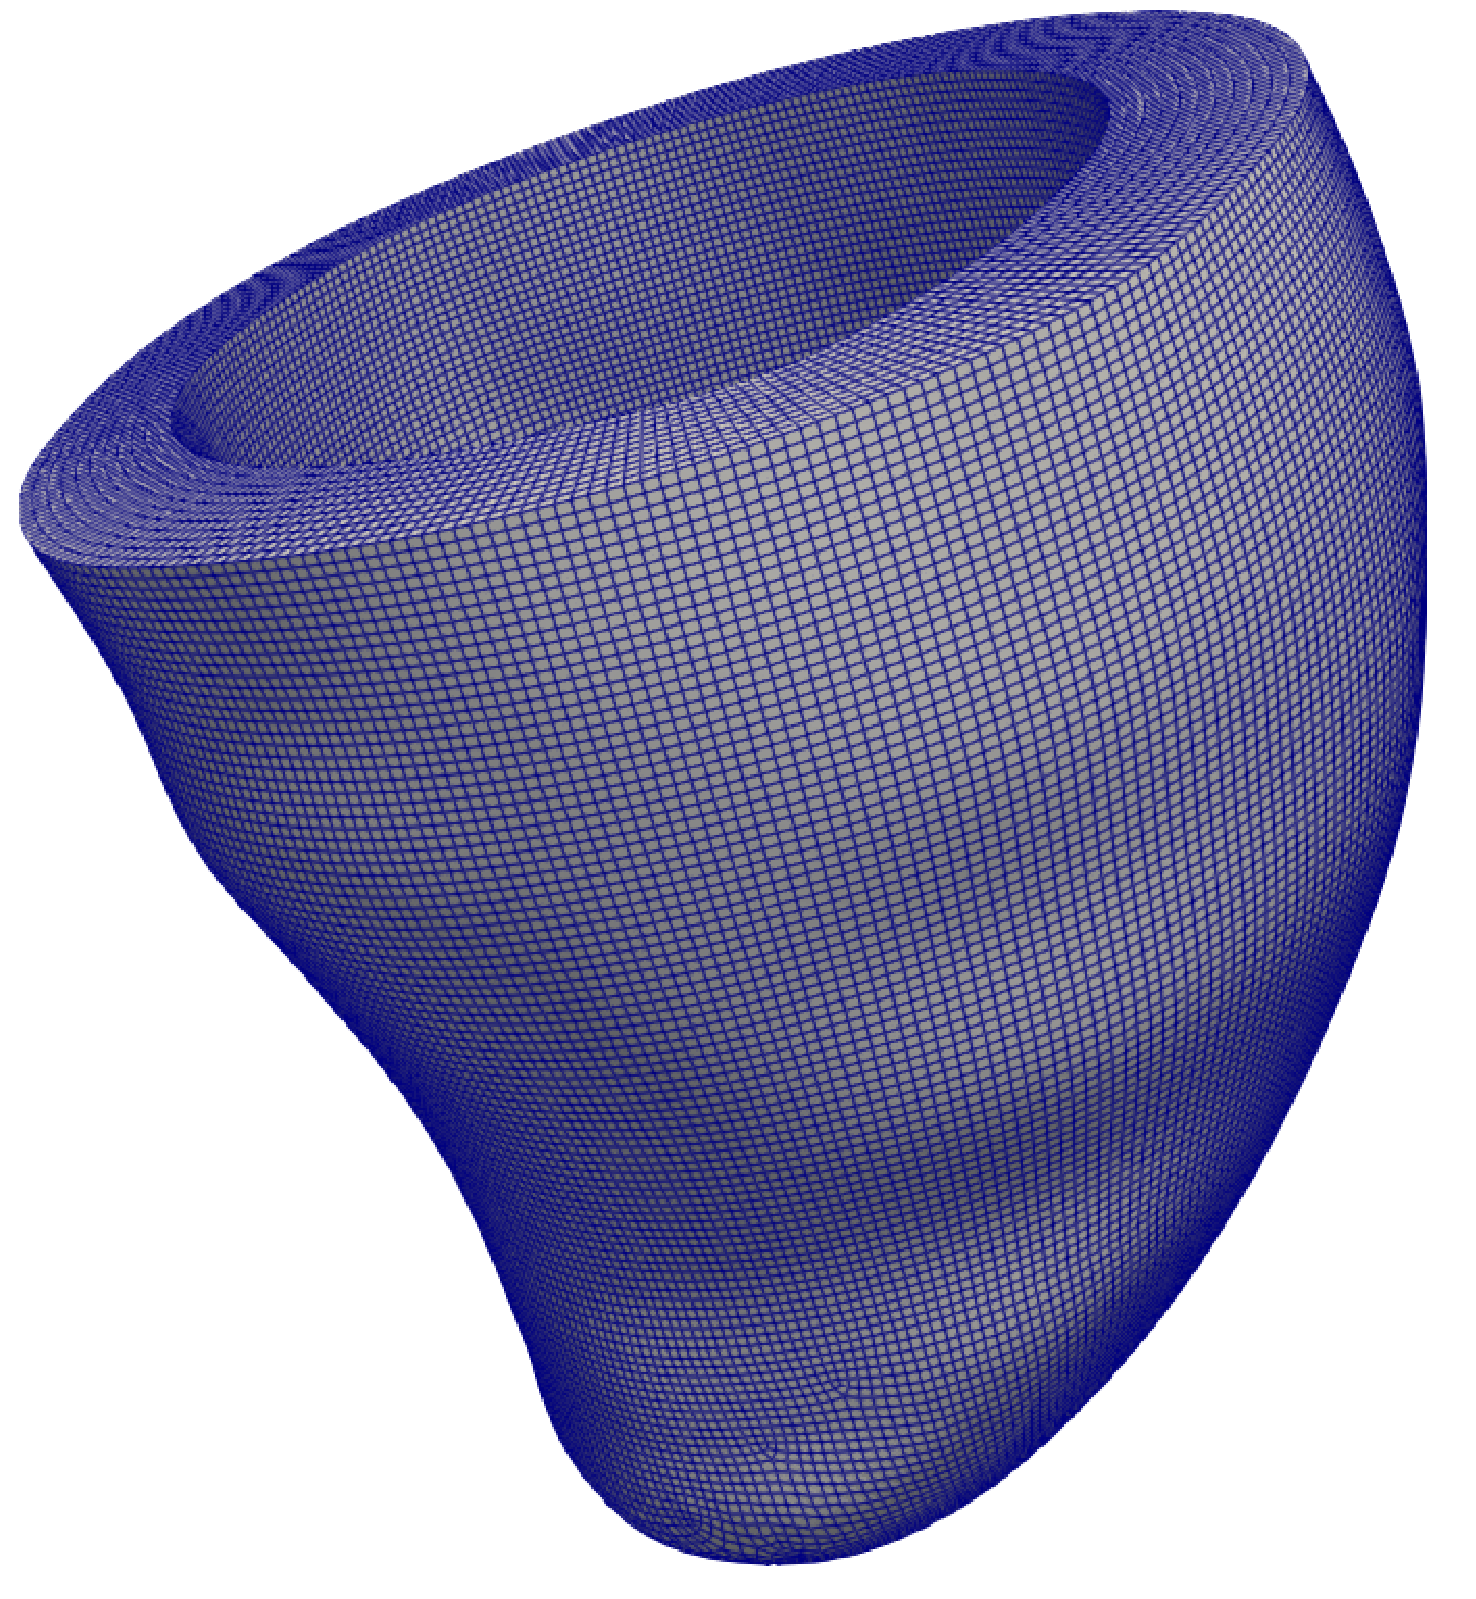
\includegraphics[width=\linewidth]{fig/left_ventricle_view-cropped.pdf}
        \caption{}
        \label{subfig:left_ventricle_mesh}
    \end{subfigure}
    \hspace{4cm}
    \begin{subfigure}{0.30\linewidth}
        \centering
        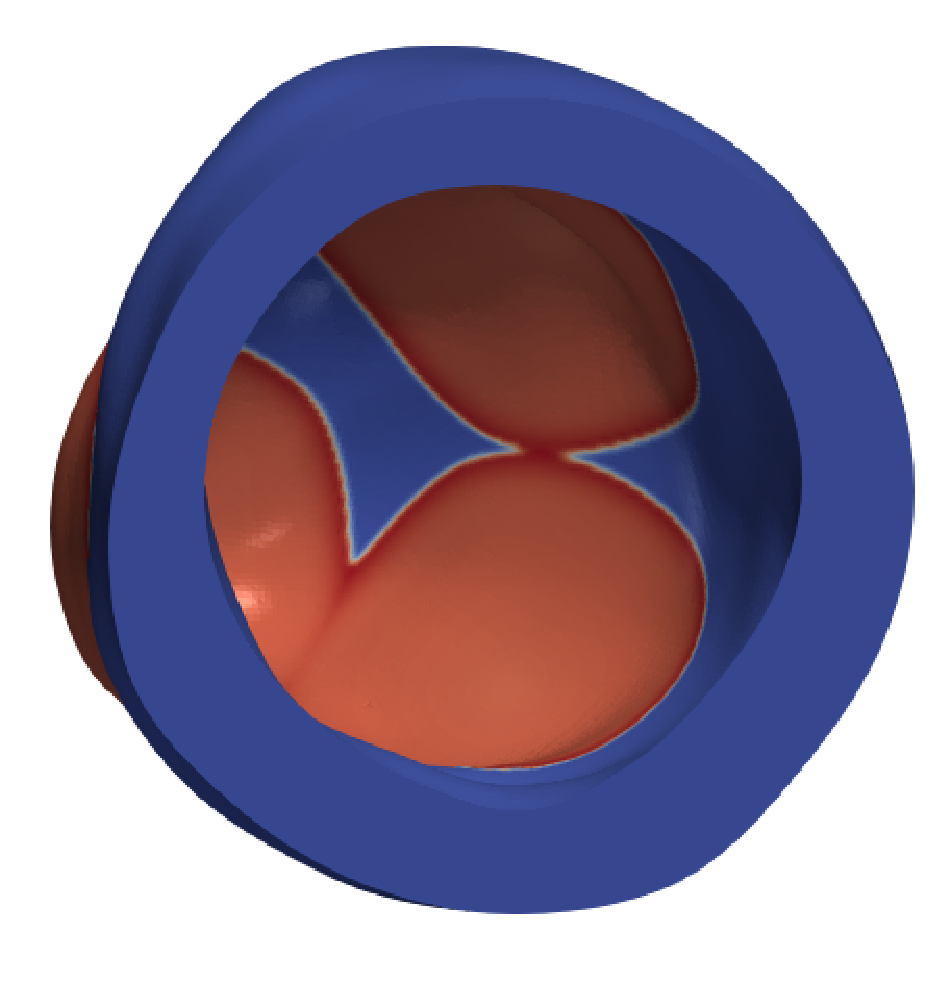
\includegraphics[width=\linewidth]{fig/view_impulses.pdf}
        \caption{}
        \label{subfig:left_ventricle_impulses}
    \end{subfigure}

    \caption{
        (\subref{subfig:left_ventricle_mesh}) Hexahedral mesh representing a realistic left ventricle.
        (\subref{subfig:left_ventricle_impulses}) Propagation of the transmembrane potential.
    }
    \label{fig:left_ventricle}
\end{figure}

\begin{figure}[h!]
    \centering
    \includegraphics[width=0.9\textwidth]{fig/iterates_3D_monodomain.pdf}
    \caption{Number of preconditioned conjugate-gradient (PCG) iterations per time step for the monodomain problem, comparing AMG and agglomerated multigrid (AggloMG) for polynomial degrees $p\!=\!1,2$ for the three-dimensional
        ventricle test.}
    \label{fig:iterates_3D_monodomain}
\end{figure}


\begin{figure}[h!]
    \centering
    \includegraphics[width=0.9\textwidth]{fig/iteration_times_3D_monodomain.pdf}
    \caption{Wall-clock time for PCG iteration time per time step for the monodomain problem, comparing AMG and agglomerated multigrid (AggloMG) for polynomial degrees $p\!=\!1,2$ for the three-dimensional
        ventricle test. Results have been obtained on 128 MPI processes on the Toeplitz cluster at University of Pisa.}
    \label{fig:iteration_times_3D_monodomain}
\end{figure}










\newpage

\section{{Integration of PSCToolkit}}
\label{sec:section5}

The integration of PSCToolkit (Parallel Sparse Computing Toolkit)~\cite{psctoolkit} aims to provide scalable algebraic
multigrid (AMG) preconditioners through its AMG4PSBLAS package. By merging the preconditioners developed within AMG4PSBLAS
into deal.II, it will be possible to exploit them as drop-in replacements in application codes. The integration
targets the following new release candidates: PSBLAS v3.9 and AMG4PSBLAS v1.2.

\subsection{Integration status}
The integration of PSCToolkit into the deal.II master branch is currently in progress, and can be tracked on the
official deal.II GitHub repository~\footnote{See \pr{19050} and \pr{18938}}. Concurrently, a fully working interface (whose code will be progressively upstreamed into the main deal.II repository) has been developed on a separate
branch\footnote{Available at \url{https://github.com/psctoolkit/dealii/commits/configure_amg4psblas/}.}, providing complete access
to the preconditioners developed within AMG4PSBLAS.

In general, the design of the user interface closely follows the existing structure of the main deal.II linear algebra frameworks, such as the
interfaces to Trilinos and PETSc. In the same fashion, the interface to AMG preconditioners by AMG4PSBLAS has been designed following the same design
principles of the existing interfaces to Trilinos and PETSc wrappers. Indeed, within the namespace \texttt{PSCToolkitWrappers}, a new class \texttt{PreconditionAMG} has been introduced, which implements
a minimal interface which allows to:
\begin{itemize}
    \item construct the preconditioner with a given set of user-specified parameters,
    \item build the AMG hierarchy and related smoothers, out of a given distributed PSBLAS system matrix,
    \item apply the resulting preconditioner to a given vector through the standardized \texttt{vmult(dst,src)} method.
\end{itemize}


Parameters are exposed by passing an \texttt{AdditionalData} object to the constructor of the preconditioner, which is a
standardized data structure to pipe additional flags to the preconditioner. In this way, the integration is completely
transparent from the user's perspective: switching from, e.g., a Trilinos ML or Hypre AMG preconditioner to an AMG4PSBLAS one requires
no structural changes to the application code.

\subsection{Preliminary results for AMG4PSBLAS preconditioners}

In order to assess the correctness and performance of our interface, we have performed a series of
numerical experiments on the cluster AMELIA. Tables~\ref{tab:amelia_2d} and~\ref{tab:amelia_3d}\todo{Add tables with AMELIA cluster results} report the
iteration counts obtained with continuous $\mathcal{Q}^1$ finite elements on quadrilateral and hexahedral meshes, respectively, for
the variable-coefficient Poisson problem
$$-\nabla \cdot ( k(x) \nabla u) = f \quad \text{ in } \Omega = [0,1]^d, \quad d=2,3,$$
with homogeneous Dirichlet boundary conditions on $\partial \Omega$. We vary the number of mesh refinement levels, the number of parallel processes, and the anisotropy of the diffusion coefficient $k(x)$, reporting on the
iteration counts of the AMG4PSBLAS preconditioner.


To evaluate performance at significantly larger problem sizes, we have been granted access to the MareNostrum 5 supercomputer at the Barcelona Supercomputing Center. These resources will enable us to conduct experiments and benchmarking at scale, providing insight into the behavior of our interface under sizes
typical of pre-exascale applications.

\subsection{Ongoing and future work}

Ongoing work includes several tasks aimed at finalizing the integration and assessing the performance of the AMG4PSBLAS preconditioners in large-scale simulations:
\begin{itemize}
    \item finalizing the interface, introducing wrappers for sparse matrix types,
    \item large-scale performance evaluations on HPC systems to identify potential performance bottlenecks in the interface and in the preconditioner itself,
    \item GPU support: PSBLAS provides GPU acceleration through CUDA backends. The exposition of this functionality through the
          deal.II interface will enable GPU-accelerated AMG preconditioning within standard deal.II solver workflows.
\end{itemize}



\newpage

\section{{Integration of MUMPS}}
\label{sec:section6}


 The direct solution of a sparse linear system $Ax=b$ relies on the factorization of the matrix $A$. 
 The robustness of direct methods comes at the cost of a high complexity both in terms
 of number of floating point operations and of memory footprint.


The complexity of the direct methods approaches can be reduced thanks to Block
Low-Rank (BLR) approximation (see \cite{ablm:17b,aabblw:15}) with adaptive precision \cite{abbg:23} to exploit data sparsity.
This is illustrated in Table~\ref{t:beltrami} on the Beltrami Flow problem from lifex library. Comparing the first two rows "Full-Rank" factorization and "BLR factorization with adaptive precision" in Table~\ref{t:beltrami} we see that the number of operation is reduce by two orders of magnitude.

\begin{table}[hb]
\begin{center}
	\begin{tabular}{|l|c|c|c|c|}
\hline
                              & {Memory used}   & Number of op. & Total time &  Backward error  \\
			      & (Gbytes) & to factor matrix & (sec) & after IR\\
\hline
  % 1 Node x 4MPI x 48th  & & & & \\
    Full-Rank                 &    {620}       &     {1.6E15}   &    {\bf 364}    &      2E-15  \\
%    BLR(1E-9)+adaptive        &    298       &     6.1E13   &    \phantom{0}57    &      4E-8\phantom{0}   \\
    BLR(1E-5)+adaptive        &    224       &     2.3E13   &    \phantom{0}38    &      1E-10   \\
%                    & & & & \\
\hline
 \multicolumn{5}{c}{ } \\
 \multicolumn{5}{c}{\bf Single precision factorization in double prec instance with mixed precision IR}  \\
\hline
       Full-Rank              &    315       &     1.6E15   &    229    &      2E-12   \\
       BLR(1E-5)+adaptive     &    {125}       &     {2.0E13}   &   \bf{\phantom{0}24}    &      8E-11  \\

\hline
\end{tabular}
\caption{\label{t:beltrami} Beltrami matrix, performance analysis, AMD Genoa (4MPI x 48th). IR=Iterative Refinement}
\end{center}
\end{table}

The performance can be further improved using mixed precision algorithms \cite{abhl22a} as illustrated with the last two lines of Table~\ref{t:beltrami}.
In row "Full-Rank", {\it single precision factorization with mixed precision iterative refinement (IR)} and an efficient approach to access data in low precision  \cite{ajlmp:2025} enable to divide time and memory by a factor of two.
Combining this approach to BLR with adaptive precision leads to an overall significant reduction in time (from 364 to 24 seconds) and memory (from 620 to 125 Gbytes) with a satisfactory backward error.
It should be mentioned, as described in \cite{abhl22a}, that on ill-conditioned matrices GMRES based iterative refinements should be used.

Recent experiments with accelerated nodes (Nvidia-GraceHopper and AMD-Mi250 and AMD-Mi300) have shown that we can reduce the time for full-rank factorization of the Beltrami matrix by a factor between 3 and 6 depending on the compute node. Next challenge will be to combine the benefits from adaptive BLR and mixed precision algorithms on accelerated nodes.





\newpage

\section{{Conclusion}} \label{sec:conclusion}

\begin{thebibliography}{10}
    \bibitem[Filippone and Colajanni, 2000]{PSBLAS}Salvatore Filippone and Michele Colajanni, "PSBLAS: a library for parallel linear algebra computation on sparse matrices", ACM Transactions on Mathematical Software, vol. 26, no. 4, pp. 527--550, 2000. \url{https://doi.org/10.1145/365723.365732}
    \bibitem[D'Ambra et al., 2025]{psctoolkit}Pasqua D'Ambra, Fabio Durastante and Salvatore Filippone, "PSCToolkit: solving sparse linear systems with a large number of GPUs", arXiv preprint arXiv:2406.19754, 2025. \url{https://arxiv.org/abs/2406.19754}
    \bibitem[Cangiani et al., 2014]{polyDG}Andrea Cangiani, Emmanuil Georgoulis and Paul Houston, "hp-Version discontinuous Galerkin methods on polygonal and polyhedral meshes," Mathematical Models and Methods in Applied Sciences, vol. 24, no. 4, pp. 2009-2041, 2014.
    \bibitem[Antonietti et al., 2013]{Antoniettihp}Paola Antonietti, Stefano Giani, and Paul Houston, "$hp$-Version Composite Discontinuous Galerkin Methods for Elliptic Problems on Complicated Domains", SIAM Journal on Scientific Computing, vol. 35, A1417-A1439, 2013.
    \bibitem[Feder et al., 2025]{FEDER2025113773}Marco Feder, Andrea Cangiani and Luca Heltai, "R3MG: R-tree based agglomeration of polytopal grids with applications to multilevel methods", Journal of Computational Physics, vol. 526, 113773, 2025.
     \bibitem[Feder and Africa, 2026]{feder2026agglomeration}Marco Feder and Pasquale Claudio Africa, "An agglomeration-based multigrid solver for the discontinuous Galerkin discretization of cardiac electrophysiology", arXiv preprint arXiv:2602.16312, 2026.
    \bibitem[Benzi et al., 2026]{BenziFederHeltai-2026-a}Michele Benzi, Marco Feder, Luca Heltai and Federica Mugnaioni, "Scalable Augmented Lagrangian preconditioners for Fictitious Domain problems", Computer methods in applied mechanics and engineering, vol. 450, p. 118522, 2026.
    \bibitem[Fehn et al., 2020]{Fehn2020}
Niklas Fehn, Peter Munch, Wolfgang A. Wall, and Martin Kronbichler, ``Hybrid multigrid methods for
  high-order discontinuous {G}alerkin discretizations'', Journal of Computational Physics, vol. 415 109538, 2020.

\bibitem[Kronbichler and Kormann, 2012]{KronbichlerKormann2012}
Martin Kronbichler and Katharina Kormann, ``A generic interface for parallel cell-based finite
  element operator application'', Computers \& Fluids 63, pp.~135--147, 2012.
\bibitem[Kronbichler and Kormann, 2019]{KronbichlerKormann}Martin Kronbichler and Katharina Kormann, ``Fast Matrix-Free Evaluation of Discontinuous Galerkin Finite Element Operators'', ACM Transactions on Mathematical Software, vol. 45, no. 3, Article 29, 2019.
\bibitem[Kronbichler and Ljungkvist, 2019]{KronbichlerLjungkvist2019}Martin
  Kronbichler and Karl Ljungkvist, ``Multigrid for matrix-free high-order
  finite element computations on graphics processors'', ACM Transactions on
  Parallel Computing 6, no. 1, Article 2, 2019.
\bibitem[Munch et al., 2023]{Munch2023}Peter Munch, Timo Heister, Laura Prieto
  Saavedra, and Martin Kronbichler, ``Efficient distributed matrix-free
  multigrid methods on locally refined meshes for FEM computations'', ACM
  Transactions on Parallel Computing, 10, no. 1, Article 3, 2023.
    \bibitem[Amestoy, Boiteau et al., 2023]{abbg:23}P.~Amestoy, O.~Boiteau, A.~Buttari, M.~Gerest, F.~Jezequel, J.-Y. L'Excellent, and T.~Mary. Mixed precision low-rank approximations and their application to block low-rank {LU} factorization. {\em IMA Journal of Numerical Analysis}, 43:2198--2227, July 2023.

    \bibitem[Amestoy, Buttari et al., 2023]{abhl22a} P.~Amestoy, A.~Buttari, N.~J. Higham, J.-Y. L'Excellent, T.~Mary, and B.~Vieubl\'e. Combining sparse approximate factorizations with mixed precision iterative refinement. {\em ACM Transactions on Mathematical Software}, 49(1):1--29, 2023.
      
    \bibitem[Amestoy et al., 2025] {ajlmp:2025} P.~Amestoy, A.~Jego, J.-Y. L'Excellent, T.~Mary, and G.~Pichon. {BLAS-based Block Memory Accessor with Applications to Mixed Precision Sparse Direct Solvers}. preprint submitted to publication, Apr. 2025.
      
    \bibitem[Amestoy et al., 2015]{aabblw:15} P.~R. Amestoy, C.~Ashcraft, O.~Boiteau, A.~Buttari, J.-Y. L'Excellent, and C.~Weisbecker. Improving multifrontal methods by means of block low-rank representations. {\em SIAM Journal on Scientific Computing}, 37(3):A1451--A1474, 2015.
      
    \bibitem[Amestoy et al., 2019]{ablm:17b} P.~R. Amestoy, A.~Buttari, J.-Y. L'Excellent, and T.~Mary. {Performance and Scalability of the Block Low-Rank Multifrontal Factorization on Multicore Architectures}. {\em ACM Transactions on Mathematical Software}, 45:2:1--2:26, 2019.

\end{thebibliography}



\label{MyLastPage}

\end{document}

%%% Local Variables:
%%% mode: LaTeX
%%% TeX-master: t
%%% End:
